\documentclass[10pt,conference]{IEEEtran}
\usepackage{cite}
\usepackage{amsmath,amssymb,amsfonts,amsthm}
\usepackage{algorithm}
\usepackage{algorithmic}
\usepackage{graphicx}
\usepackage{textcomp}
\usepackage{xcolor}
\usepackage[hyphens]{url}
\usepackage{fancyhdr}
\usepackage{hyperref}
\hypersetup{hidelinks}
\usepackage{booktabs}
\usepackage{multirow}
\usepackage{array}
\usepackage{balance}
\usepackage{siunitx}
\usepackage{placeins}

\pdfpagewidth=8.5in
\pdfpageheight=11in
\newcommand{\hpcayear}{2027}
\newcommand{\hpcasubmissionnumber}{1467}
\title{XORFLOW: Online Inter-Layer Support Compression for Deep Residual GNN Accelerators}

% Camera-ready fields remain unused for double-blind submission.
%\def\hpcacameraready{}
\newcommand{\hpcapubid}{}
\newcommand\hpcaauthors{Anonymous Authors}
\newcommand\hpcaaffiliation{Anonymous Institution}
\newcommand\hpcaemail{anonymous@example.com}
\input{hpca-template}

\newcommand{\sys}{\textsc{XORFLOW}}
\newcommand{\beicsr}{\textsc{BEICSR}}
\newcommand{\Azero}{\textsc{A0}}
\newcommand{\Atwo}{\textsc{A2}}
\newcommand{\DeltaFmt}{\textsc{Delta}}
\newcommand{\xor}{\mathbin{\oplus}}
\newcommand{\argminpref}{\operatorname*{arg\,min}}
\newtheorem{proposition}{Proposition}
\newtheorem{lemma}{Lemma}

\begin{abstract}
Deep residual graph neural networks repeatedly materialize sparse intermediate features, making activation movement a major off-chip cost. This paper presents \sys, an online lossless representation that exploits positional persistence between adjacent post-ReLU supports. \sys{} independently encodes an anchor support and represents the following support by an XOR event stream only when the complete delta record is smaller than independent encoding. Across ten compatible eight-layer checkpoints, \sys{} reduces serialized support writes by 37.1\% and complete physical traffic by 7.9\%, yielding 1.083$\times$ trace-weighted geometric-mean modeled subsystem speedup. On valid deeper configurations, the modeled subsystem speedup reaches \textbf{1.324$\times$} on Reddit D16. Byte-exact reconstruction, finite-capacity producer/consumer scheduling, external memory replay, RTL co-simulation, and physical implementation substantiate the representation and datapath.\\
Anonymous artifact: \url{https://anonymous.4open.science/r/HPCA-2-0315/}.
\end{abstract}

\section{Introduction}

Graph neural networks (GNNs) alternate irregular neighborhood aggregation with dense feature transformation. This execution pattern has led to specialized accelerators with separate sparse and dense engines~\cite{yan2020hygcn,li2021gcnax,hwang2023grow}. Deep residual GNNs add another pressure point: every block produces a large intermediate node--feature matrix that must remain available to the next block. As depth grows, these intermediate tensors create a repeated stream of off-chip writes and reads.

ReLU makes many intermediate values zero. A sparse accelerator stores the remaining values together with a \emph{support}, the binary map that identifies their node--feature positions. Prior feature formats, including \beicsr{} in SGCN~\cite{yoo2023sgcn}, reduce this traffic by compressing each support separately. That approach exploits sparsity inside one layer but ignores how the support changes from one residual block to the next.

The key observation behind \sys{} is that adjacent residual layers often preserve the location of active features. Only a smaller set of positions switches between zero and nonzero. This creates an inter-layer representation opportunity: retain one independently decodable support and encode the next support as the positions that changed. The idea is simple algebraically, but an online accelerator must solve four concrete problems. The first support must be committed before the second exists; the retained support still needs compact storage; an XOR difference can expand on weakly related regions; and reconstruction must complete before sparse aggregation requests the packed values.

\sys{} solves these problems with a two-stage representation and a matching dataflow. Supports are partitioned into row \emph{tiles} and feature \emph{slices}; a tile/slice is the unit independently selected and decoded. The first support in a pair is the \emph{anchor}. \sys{} selects the smallest independently decodable anchor among \beicsr, row events, and a majority-prototype codec. The next support is the \emph{target}. Its changed positions form an XOR \emph{delta}; \sys{} selects the delta only when its complete serialized record is smaller than an independent \beicsr{} target. Parallel decoders reconstruct a tile-local bitmap that directly gates packed-value reads.

The resulting mechanism is not tied to one host accelerator. It is a support-stream representation and producer/consumer dataflow that can be inserted wherever sparse intermediate features are written and later consumed. The evaluation uses an optimized \beicsr{} implementation as the direct numerical baseline because it encodes the same support stream under identical caches, memory, precision, and compute resources. Dense bitmap, CSR variants, independent event coding, spatial prototypes, forced deltas, residual/non-residual models, depth, width, and memory-system sweeps isolate the source and limits of the gain.

This paper makes four contributions:
\begin{itemize}
  \item \textbf{Inter-layer support characterization.} Across 26 traced configurations, adjacent supports reach median Jaccard 0.879 and exception density 0.0588; exact-count independent controls fall to 0.327 and rise to 0.4925, respectively.
  \item \textbf{Online anchor--delta representation.} \sys{} combines a Hamming-optimal majority prototype, exact XOR reconstruction, and local fallback. The anchor decision never reads a future layer, and the serialized pair-write cost is bounded by \beicsr{} using the same record partition and slice width; the evaluation separately compares independently optimized \beicsr{} widths.
  \item \textbf{GNN support-stream microarchitecture.} A producer-side cohort engine performs majority construction, XOR event discovery, exact Dense/ID/Gap8 packing, and local format selection. Parallel variable-length decoders, event scatter, and banked support construction expose reconstructed supports to sparse aggregation.
  \item \textbf{Architecture-faithful system evaluation.} Byte-exact records, complete producer and consumer anchor accounting, all ten eligible checkpoints, a shared eight-channel read/write memory model, SCALE-Sim combination service, held-out Ramulator2 validation, producer co-simulation, bank-aware decoder modeling, and integrated-cluster routing quantify both benefit and cost.
\end{itemize}

\section{Preliminaries}

\subsection{Residual GNN execution}
Let $G=(V,E)$ be a graph with $N=|V|$ nodes. Layer $\ell$ consumes $H^{(\ell)}\in\mathbb{R}^{N\times F_\ell}$ and computes
\begin{equation}
H^{(\ell+1)}=\phi\!\left(\widehat{A}H^{(\ell)}W^{(\ell)}+R^{(\ell)}\right),
\label{eq:gnn}
\end{equation}
where $\widehat{A}$ is the normalized sparse adjacency operator, $W^{(\ell)}$ is the dense transform, $R^{(\ell)}$ is the residual branch, and $\phi$ applies normalization and ReLU~\cite{ba2016layernorm}. Aggregation traverses graph edges and reads features irregularly; combination applies $W^{(\ell)}$ on dense arrays.

The \emph{support} of a post-ReLU feature matrix is the binary matrix
\begin{equation}
S_\ell[v,f]=\mathbf{1}\!\left[H^{(\ell)}[v,f]\neq0\right].
\label{eq:support}
\end{equation}
The nonzero values are stored densely in a packed stream, while the support tells aggregation which values exist. Existing layer-local formats reduce the size of $S_\ell$ but encode $S_\ell$ and $S_{\ell+1}$ independently.

\subsection{Inter-layer support transitions}
For adjacent supports, define the transition support
\begin{equation}
D_\ell=S_\ell\xor S_{\ell+1}.
\label{eq:delta}
\end{equation}
A one in $D_\ell$ is an \emph{event}: one node--feature position changed between layers. The representation developed below encodes these events when doing so is smaller than independently encoding the target support.

\section{XORFLOW Representation}
\label{sec:representation}

\subsection{Tiles, slices, anchors, and targets}
Reverse Cuthill--McKee reorders nodes once for storage locality and is applied identically to every format~\cite{george1971rcm}. Each support is divided into row tiles of $R=128$ nodes and feature slices of width $C$. For tile $t$ and slice $q$, $S_\ell^{t,q}\in\{0,1\}^{R\times C}$ is one independently encoded record.

Non-overlapping layer pairs are indexed by $p$:
\begin{equation}
A_p=S_{2p}^{t,q},\qquad T_p=S_{2p+1}^{t,q},\qquad D_p=A_p\xor T_p,
\label{eq:pair}
\end{equation}
where $A_p$ is the anchor, $T_p$ is the target, and $D_p$ is their event map. An unpaired final support is encoded independently.

\subsection{Hardware-oriented event coding}
Let $E\subseteq\{0,\ldots,U-1\}$ contain $k$ sorted events from a universe of $U$ positions. Let $w(U)=\lceil\log_2U\rceil$ and $c(U)=\lceil\log_2(U+1)\rceil$. Ignoring record-wide fields common to all three choices, the event payload uses the minimum of
\begin{align}
L_{\mathrm{dense}}(U)&=U,\label{eq:dense}\\
L_{\mathrm{id}}(U,k)&=c(U)+k\,w(U),\label{eq:id}\\
L_{\mathrm{gap}}(U,k,b)&=9+b\,[w(U)+5]+8(k-b),\label{eq:gap}
\end{align}
where $b$ is the number of Gap8 blocks. Dense mode emits a bitmap; ID mode emits fixed-width sorted positions; Gap8 emits one restart identifier and up to 31 positive 8-bit gaps per block. The selector chooses the shortest emitted payload after byte rounding. In particular, ID mode beats a dense bitmap whenever
\begin{equation}
k < \frac{U-c(U)}{w(U)},
\label{eq:idthreshold}
\end{equation}
which formalizes why sparse transition events are compact even when the anchor itself is not sparse.

\subsection{Independent anchor coding}
The anchor must be written before $T_p$ exists. \sys{} therefore compares three independently decodable records.

\textbf{\beicsr} stores the layer-local bitmap used by the direct baseline. \textbf{\Azero} applies Eqs.~\ref{eq:dense}--\ref{eq:gap} to the set positions of each row. \textbf{\Atwo} partitions up to $g=32$ rows into a cohort, stores one prototype $P\in\{0,1\}^{C}$, and event-encodes each residual row $A_p[r,:]\xor P$.

The prototype minimizes residual Hamming count. For cohort rows $x_1,\ldots,x_g$, define the residual event count
\begin{equation}
E(P)=\sum_{r=1}^{g}\lVert x_r\xor P\rVert_0.
\label{eq:prototypeobjective}
\end{equation}

\begin{proposition}[Hamming-optimal majority prototype]
Let $n_j=\sum_{r=1}^{g}x_r[j]$. The bitwise majority
\begin{equation}
P^*[j]=\mathbf{1}[n_j>g/2]
\label{eq:majority}
\end{equation}
minimizes $E(P)$, with deterministic zero ties, and
\begin{equation}
E(P^*)=\sum_{j=1}^{C}\min(n_j,g-n_j)\le \frac{gC}{2}.
\label{eq:majoritybound}
\end{equation}
\end{proposition}
\begin{proof}
Equation~\ref{eq:prototypeobjective} separates by feature column. Choosing $P[j]=0$ creates $n_j$ residual events; choosing $P[j]=1$ creates $g-n_j$. The smaller choice is the majority value, yielding $\min(n_j,g-n_j)$ events for column $j$. Summing over columns proves optimality. Since each minimum is at most $g/2$, the total is at most $gC/2$.
\end{proof}
The proposition optimizes the number of residual events, not the nonlinear serialized-byte objective after Dense/ID/Gap8 selection and byte rounding. \sys{} therefore calls the prototype Hamming-optimal rather than byte-optimal. The majority construction is a one-pass, column-separable hardware rule with the event-count bound in Eq.~\ref{eq:majoritybound}; complete serialized lengths are still compared after every candidate is emitted.

Let $B_F(X)$ denote the complete 64-byte-aligned serialized length of support $X$ under format $F$, including its record header and variable-length fields. The anchor selector is
\begin{equation}
F_A=\argminpref_{F\in\{\beicsr,\Azero,\Atwo\}} B_F(A_p),
\label{eq:anchorselect}
\end{equation}
with ties resolved in favor of \beicsr. The selected anchor is committed immediately.

\subsection{Target delta and local fallback}
When $T_p$ is produced, the encoder obtains $A_p$ from the anchor buffer or a charged memory reread and forms $D_p$. The target choice is
\begin{equation}
F_T=
\begin{cases}
\DeltaFmt, & B_{\DeltaFmt}(D_p)<B_{\beicsr}(T_p),\\
\beicsr, & \text{otherwise}.
\end{cases}
\label{eq:targetselect}
\end{equation}
The delta is therefore used only where its complete serialized record is beneficial.

\begin{proposition}[Fixed-partition serialized pair-write bound]
Fix the same tile boundaries, slice width, record headers, and alignment policy for \sys{} and \beicsr{}. The serialized support writes for every pair satisfy
\begin{equation}
B_{\mathrm{XF}}(A_p,T_p)\le B_{\mathrm{BEI}}^{(q)}(A_p)+B_{\mathrm{BEI}}^{(q)}(T_p),
\label{eq:noexpand}
\end{equation}
where $q$ denotes that common partition and slice width.
\end{proposition}
\begin{proof}
Under the fixed layout $q$, the candidate set in Eq.~\ref{eq:anchorselect} contains \beicsr, so the selected anchor is no larger than $B_{\beicsr}^{(q)}(A_p)$. The target candidate set in Eq.~\ref{eq:targetselect} also contains \beicsr, so the selected target is no larger than $B_{\beicsr}^{(q)}(T_p)$. Adding the two inequalities proves Eq.~\ref{eq:noexpand}.
\end{proof}
The bound applies only to serialized support writes under one fixed layout. It neither compares against the independently optimized per-workload \beicsr{} width nor bounds reads, packed values, topology, output writes, or cache effects. Those quantities are evaluated separately.

\subsection{Exactness, causality, and bounded state}
A delta target reconstructs as
\begin{equation}
A_p\xor D_p=A_p\xor(A_p\xor T_p)=T_p.
\label{eq:exact}
\end{equation}
The anchor decision is a function of $A_p$ alone and completes before $T_p$ is available. The target decision reads only the committed anchor and current target. The producer and consumer have distinct anchor lifetimes. The producer retains or reconstructs $A_p$ until $T_p$ has been encoded; the consumer must later obtain $A_p$ again before decoding a \DeltaFmt{} target. No record refers beyond its pair, so the dependency does not form a multi-layer chain, but the consumer-side anchor source must be explicit and timing-active.

\begin{algorithm}[t]
\caption{Online encoding of one tile/slice stream}
\label{alg:online}
\begin{algorithmic}[1]
\REQUIRE Supports $S_0,S_1,\ldots$ in production order
\FOR{$\ell=0,1,\ldots$}
  \IF{$\ell$ is even}
    \STATE $A\leftarrow S_\ell$
    \STATE build \beicsr$(A)$ and \Azero$(A)$
    \STATE for each 32-row cohort, compute $P^*$ by Eq.~\ref{eq:majority}
    \STATE build \Atwo$(A)$ from $P^*$ and row residual events
    \STATE commit the shortest of \beicsr$(A)$, \Azero$(A)$, and \Atwo$(A)$
    \STATE retain $A$ subject to anchor-buffer capacity
  \ELSE
    \STATE obtain anchor $A$; charge a memory read on a miss
    \STATE $D\leftarrow A\xor S_\ell$
    \STATE build \DeltaFmt$(D)$ using Eqs.~\ref{eq:dense}--\ref{eq:gap}
    \STATE build independent \beicsr$(S_\ell)$
    \STATE commit the shorter target record; prefer \beicsr{} on a tie
    \STATE release $A$
  \ENDIF
\ENDFOR
\end{algorithmic}
\end{algorithm}

\begin{figure*}[t]
\centering
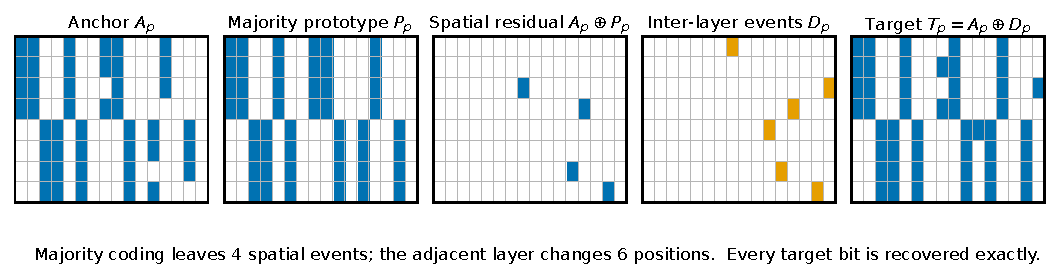
\includegraphics[width=\textwidth]{figures/fig2_exact_example.pdf}
\caption{Bit-exact example. The majority prototype minimizes the four anchor residual events. Six inter-layer events form $D_p$, and XOR with the committed anchor reconstructs $T_p$ exactly.}
\label{fig:example}
\end{figure*}

\subsection{Serialized record}
Each record begins with a 16-bit little-endian header containing a 2-bit format tag and a 14-bit payload-byte count. Payload integers are unsigned and emitted least-significant-bit first. An event payload begins with a 2-bit mode. Dense mode emits $U$ bits; ID mode emits a $c(U)$-bit count and $w(U)$-bit identifiers; Gap8 emits a 9-bit block count, then for each block a $w(U)$-bit restart identifier, a 5-bit length-minus-one, and positive 8-bit gaps. \Atwo{} emits one $C$-bit prototype per cohort followed by residual event payloads. A 16-byte offset table locates variable-length records, and every record is zero-padded to 64 bytes. The decoder rejects reserved tags, truncated fields, zero gaps, unsorted or out-of-range identifiers, inconsistent counts, dimension mismatches, and nonzero padding.

The serialized format is self-delimiting and byte-exact: analytical field lengths match emitted records, and decoding reconstructs each support without reference to layers outside its anchor--target pair.

\section{Microarchitecture and Performance Model}

\begin{figure*}[t]
\centering
\fbox{\begin{minipage}[c][1.30in][c]{0.96\textwidth}
\centering\large\textbf{Figure 2 placeholder}\\[3pt]
\normalsize Final producer--consumer microarchitecture artwork will be inserted here.
\end{minipage}}
\caption{Placeholder for the final \sys{} producer and consumer microarchitecture.}
\label{fig:architecture}
\end{figure*}

\subsection{Producer-side encoder}
The write path in Figure~\ref{fig:architecture} receives the post-ReLU support tile while packed values follow the ordinary output path. For an anchor, parallel generators construct \beicsr, \Azero, and \Atwo{} records and their exact byte counts. For a target, independent \beicsr{} generation runs beside anchor XOR, event discovery, and \DeltaFmt{} packing. A byte selector commits the minimum record, and the output FIFO issues 64-byte-aligned memory writes.

The bounded cohort kernel captures a $32\times64$-bit support region, accumulates the majority prototype, scans all 2,048 positions, and constructs Dense, ID, and Gap8 streams. Twenty-four reference records spanning empty, dense, majority-tie, Gap8-boundary, diagonal, and randomized inputs match the software serializer byte-for-byte under randomized stalls. The selector/ready--valid boundary maps to 810 Yosys cells, and the segmented tile-record engine maps to 1,055 cells. This mapped unit performs event discovery, exact candidate-length selection, descriptor offsets, and finite ready/valid output for one 2,048-bit tile record. Producer service and backpressure are included in the capacity-constrained execution model.

\subsection{Producer and consumer anchor lifecycles}
Every \DeltaFmt{} target uses the uncompressed anchor bitmap twice. The producer needs $A_p$ before forming $D_p=A_p\xor T_p$; the consumer later needs the same $A_p$ before reconstructing $T_p=A_p\xor D_p$. The two lifecycles have separate buffers, reads, decode service, and readiness conditions.

A default $128\times128$ tile/slice contains $RC=16{,}384$ support bits, or 2~KiB. Both evaluated stores use record identifiers and least-recently-used replacement. A producer entry is live from anchor production until target encoding. A consumer entry is inserted after anchor decode and remains live until the paired target completes or eviction. Let $h_p^P$ and $h_p^C$ denote producer and consumer hits. A miss rereads the exact padded committed anchor record and decodes it:
\begin{align}
R_p^P&=(1-h_p^P)\,64\left\lceil B_{F_A}(A_p)/64\right\rceil,\\
R_p^C&=(1-h_p^C)\,64\left\lceil B_{F_A}(A_p)/64\right\rceil,\label{eq:anchorbytes}\\
C_p^x&=(1-h_p^x)\left[C_{\mathrm{mem}}(R_p^x)+C_{\mathrm{adec}}(F_A,A_p)\right].
\label{eq:anchorcycles}
\end{align}
Here $x\in\{P,C\}$. An independently encoded target requires neither consumer anchor read nor reconstruction XOR.

Across all evaluated traces, the lifecycle accounting classifies 72,604 \DeltaFmt{} targets: 422 find a decoded consumer anchor and 72,182 reread the committed record. At 16~KiB, the consumer therefore has a 0.581\% hit rate, rereads 149.60~MB (142.67~MiB), and performs 1.320 million anchor-decode cycles. Producer accounting reconciles to the same 149.60~MB and 1.320 million cycles; together the two lifecycles charge 299.20~MB and 2.641 million decode cycles. Increasing the consumer store to 256~KiB, 1~MiB, and 4~MiB raises hit rate to 7.10\%, 27.94\%, and 80.43\%, while reread traffic falls to 133.46, 103.92, and 28.61~MiB. The store is bounded pair state rather than a conventional high-reuse cache: each anchor serves one paired target, and large graphs stream many records between production and consumption.

The final unified event trace contains 73,652 target records and verifies the complete lifecycle ordering. On every producer miss, the anchor reread completes and the anchor decode finishes before target XOR and serialization begin; the minimum memory-to-decode and decode-to-encode slack is nonnegative, with zero violations. On the consumer path, target reconstruction waits for both the complete target payload and the decoded anchor, and sparse aggregation waits for support-cache completion. Producer and consumer reread bytes and decode cycles reconcile exactly with the per-record trace.

\subsection{Parallel reconstruction}
The read path contains four eight-lane clusters. Each 64-bit lane parses one record, expands event positions, applies a prototype or anchor XOR, and emits support-word updates. The stream router distributes variable-length records; event-scatter logic maps updates to cache words; same-word updates are merged before finite bank arbitration. A 16-KiB banked cache holds reconstructed tile supports. A row prefix is the cumulative number of set support bits before a row; it converts a support position into its offset in the packed-value stream. Aggregation requests packed values only after the corresponding support row and prefix are ready.

The cycle model includes finite lane FIFOs, stream imbalance, event scatter, bank conflicts, same-word merging, SRAM-port constraints, and downstream ready/valid backpressure. In the bank sweep, median achieved throughput rises from 949.6 encoded bits/cycle with eight banks to 1,559.1 with 16 banks and 1,822.4 with 32 banks; conflicts fall by 97.1\% relative to eight banks and lane utilization reaches 89.0\%. An integrated eight-lane decoder/support-cache top passes Verilator co-simulation and routes in OpenROAD/Nangate45 at a 1.0-ns target with +0.565-ns slack, zero detailed-route DRC errors, and a 0.0682~mm$^2$ die. Supplementary Fig.~S4 reports the encoder queue and decoder-bank surfaces.

\subsection{Capacity-enforcing execution schedule}
\label{sec:timingstatus}
For record $i$ at stage $j$, let $r_j(i)$ be data readiness, $w_j(i)$ the earliest resource-availability time, and $q_j(i)$ the time at which finite downstream capacity becomes available. The schedule uses
\begin{align}
s_j(i)&=\max\{r_j(i),w_j(i),q_j(i)\},\\
f_j(i)&=s_j(i)+L_j(i).
\label{eq:queuerecurrence}
\end{align}
Target encoding waits for both the produced target support and the producer anchor,
\begin{equation}
r_E(i)=\max\{f_{\mathrm{support}}(i),f_{\mathrm{anchor}}^P(i)\},
\label{eq:producerready}
\end{equation}
and a \DeltaFmt{} target waits for the complete target record and decoded consumer anchor,
\begin{equation}
r_D(i)=\max\{f_{\mathrm{desc}}(i),f_{\mathrm{payload}}(i),f_{\mathrm{anchor}}^C(i)\}.
\label{eq:consumerready}
\end{equation}
Input, producer, decode, aggregation, combination, and writeback queues have depth four and block their producers when full. Layer $\ell+1$ cannot consume data until every write from layer $\ell$ completes.

One persistent memory resource spans the full run and is shared by producer-anchor reads, target and consumer-anchor reads, and output writebacks. A 32-entry request queue is distinct from eight timing-active channel slots. Each 64-byte record is deterministically striped by physical address; a channel transfers 32~bytes/cycle, applies a 50-cycle callback latency, and charges eight cycles when direction changes between reads and writes. This model intentionally abstracts bank and row scheduling. A calibration trace sets the timing scale, and an independent held-out trace differs from Ramulator2 by 0.45\% (Section~\ref{sec:memoryvalidation}). Thus the event graph captures shared read/write contention and finite admission, while the external simulator checks the banked HBM timing abstraction.

Combination service is not inferred from row count. Every executed record looks up a SCALE-Sim~\cite{samajdar2018scalesim} entry for a 32$\times$32 weight-stationary array using its $(M,K,N)$ feature shape. Seven unique shapes cover the evaluated records; the cache records dimensions, cycles, prefetch cycles, utilization, and a SHA-256 key. Baseline and \sys{} consume the same per-shape table. An independent max-plus implementation reproduces all baseline and proposal schedules across the twelve reported configurations.

\subsection{From compressed bytes to speedup}
Let the baseline physical traffic be $T_B=T_o+T_s$, where $T_s$ is support traffic and $T_o$ is unchanged topology, value, descriptor, and output traffic. If support encoding reduces $T_s$ by fraction $\rho$ and anchor rereads add $T_r$, then
\begin{equation}
\tau=1-\frac{T_X}{T_B}=\alpha\rho-\delta,
\quad
\alpha=\frac{T_s}{T_B},\quad
\delta=\frac{T_r}{T_B}.
\label{eq:trafficbound}
\end{equation}
Thus a large support reduction produces a large total reduction only when support occupies a meaningful fraction of physical traffic and rereads remain small.

Let $C_B=C_{\mathrm{fixed}}+C_{\mathrm{mem}}$ be baseline subsystem cycles. Let $\mu=C_{\mathrm{mem}}/C_B$ be the fraction exposed to traffic reduction, and let $\epsilon=C_{\mathrm{codec}}/C_B$ be encoding, decoding, and added stall cost. A serial conservative model gives
\begin{equation}
\mathrm{Speedup}
=\frac{C_B}{C_{\mathrm{fixed}}+(1-\tau)C_{\mathrm{mem}}+C_{\mathrm{codec}}}
=\frac{1}{1-\mu\tau+\epsilon}.
\label{eq:speedupmodel}
\end{equation}
The necessary and sufficient break-even condition in this model is
\begin{equation}
\mu\tau>\epsilon.
\label{eq:breakeven}
\end{equation}
This relation predicts the evaluation trends: depth raises the amount of reusable support traffic, narrow slices suffer fixed record overhead, and very wide layers can reduce bytes while dense combination lowers $\mu$ and hides the latency benefit.

The cycle evaluation reports the aggregation--combination subsystem under Eq.~\ref{eq:queuerecurrence}. Baseline and \sys{} use the same queue capacities, barriers, and compute resources. The reported timing result is
\begin{equation}
\mathrm{Speedup}=\frac{C_B}{C_X},
\label{eq:cycles}
\end{equation}
where $C_B$ and $C_X$ are the corrected baseline and \sys{} completion times from the same finite-queue event graph.

\section{Evaluation Methodology}

\subsection{Workloads}
The principal architecture is an eight-layer, width-128 residual GCN with LayerNorm--ReLU--GCN ordering. The primary evaluation contains ten checkpoints spanning Flickr, OGBN-Arxiv, Reddit, and Yelp, with three independent runs for each of the first three datasets and one for Yelp. Additional traces vary depth, width, residual structure, GNN operator, and graph. Supports are captured after FP8 E4M3 quantization in layer-production order, and paired FP32 versus FP8/FP16 quality uses the same checkpoint and run.

All ten primary checkpoints use the same optimized baseline, serializer, producer/consumer anchor policy, finite queues, shared eight-channel memory resource, SCALE-Sim table, and hardware service rates. A 16-layer Arxiv model and Chameleon negative control use the same scheduler but are reported separately from the primary aggregate.

\begin{table}[t]
\centering
\caption{Primary datasets and input dimensions.}
\label{tab:datasets}
\footnotesize
\begin{tabular}{lrrrr}
\toprule
Dataset & Nodes & Edges & Input features & Classes \\
\midrule
Reddit & 232,965 & 114,615,892 & 602 & 41 \\
OGBN-Arxiv & 169,343 & 1,166,243 & 128 & 40 \\
Flickr & 89,250 & 899,756 & 500 & 7 \\
Yelp & 716,847 & 13,954,819 & 300 & 100 \\
\bottomrule
\end{tabular}
\end{table}

\subsection{Baselines and common host}
All comparisons use the same traces, node order, FP8/FP16 arithmetic, cache hierarchy, memory transactions, topology stream, and compute resources. The primary baseline independently selects the best \beicsr{} slice width from 64, 96, 128, and 256 features per workload. Dense bitmap, CSR variants, independent row events, independent majority prototypes, fixed-anchor XOR, generic XOR--gap coding, forced delta, and full \sys{} provide matched representation comparisons. A noncausal pair oracle is used only as an upper-bound diagnostic.

The modeled host runs at 1~GHz with eight aggregation engines, eight dense combination arrays, a 512-KiB feature cache, and a 16-KiB support cache. Eight HBM2 channels provide a nominal 256~GB/s with 32-byte transactions. The default support record is $128\times128$ bits, and the logical decoder contains four clusters of eight 64-bit lanes.

\subsection{Metrics and validation}
Support bytes are exact emitted records. Physical traffic includes topology, packed values, support records, descriptors, output writes, and compressed-anchor reads on both the producer and consumer paths. The unified accounting charges both producer and consumer compressed-anchor reads. Support and lifecycle bytes are exact emitted-record quantities; subsystem cycles come from the common finite-queue event graph described above. The result package contains per-trace absolute cycles, dependency and queue audits, the SCALE-Sim shape cache, RTL co-simulation, synthesis, routing, and held-out external-memory validation. Ramulator2~\cite{luo2024ramulator2} provides the absolute HBM completion check, while DRAMsim3~\cite{li2020dramsim3} independently verifies complete request service under a second mapping. Yosys, Verilator, OpenROAD~\cite{kahng2019openroad}, and CACTI~\cite{muralimanohar2009cacti} provide implementation evidence.

\section{Evaluation}

\subsection{Inter-layer support persistence}
\begin{figure*}[t]
  \centering
  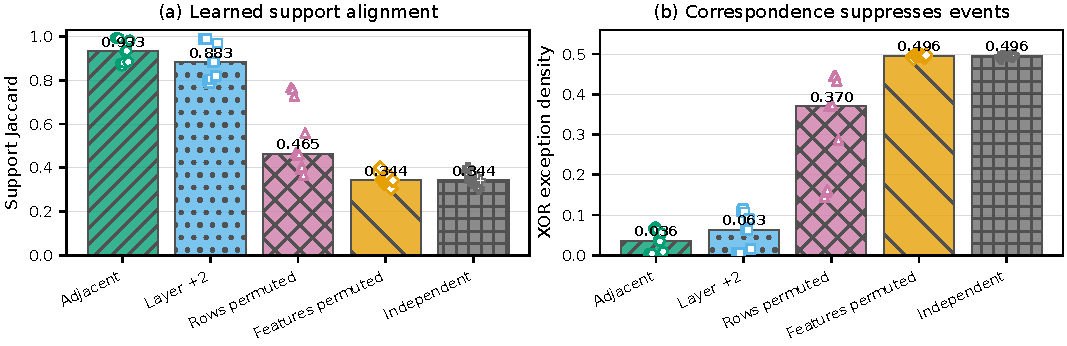
\includegraphics[width=\textwidth]{figures/fig1_opportunity_scaling.pdf}
  \caption{Inter-layer support persistence. (a) Real adjacent supports preserve substantially more active positions than nonadjacent, row-permuted, feature-permuted, and exact-count independent controls. (b) Destroying correspondence raises XOR exception density. Bars show medians across the ten compatible eight-layer checkpoints; markers show individual checkpoints. Full 26-trace distributions and layerwise results appear in Supplementary Fig.~S1.}
  \label{fig:opportunity}
\end{figure*}

Figure~\ref{fig:opportunity}(a--b) isolates positional persistence from sparsity. Across the ten primary checkpoints, real adjacent pairs reach median support Jaccard 0.933 and exception density 0.0356. Exact-count independent masks preserve each support's number of ones but reduce median Jaccard to 0.344 and raise exception density to 0.496. Row permutation raises exception density to 0.370 and causes independent encoding to be selected for essentially every record. Across the broader 26-trace suite, the corresponding medians are 0.879 versus 0.327 and 0.0588 versus 0.4925. The delta advantage therefore derives from learned positional correspondence rather than density alone; Supplementary Fig.~S1 reports the complete distributions and layerwise progression.

\subsection{Anchor accounting and dependency audit}
\begin{figure*}[t]
  \centering
  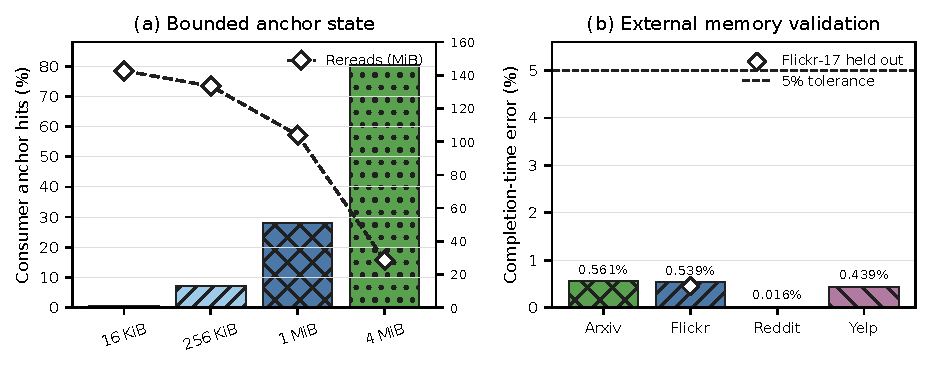
\includegraphics[width=\textwidth]{figures/fig8_final_validation.pdf}
  \caption{Online and timing validation. (a) Larger anchor stores reduce exact compressed rereads, although each anchor has only one paired target. (b) Cross-workload complete retained-stream replay remains within 0.57\% of Ramulator2; the overlaid Flickr--17 marker is an independent held-out absolute check at 0.45\%. All are below the predeclared 5\% tolerance.}
  \label{fig:onlinevalidation}
\end{figure*}

Figure~\ref{fig:onlinevalidation}(a) shows that the 16-KiB consumer store retains only 0.581\% of delta anchors. Every miss rereads a compressed committed record rather than an uncompressed 2-KiB bitmap. Increasing capacity to 4~MiB raises the hit rate to 80.43\% and lowers consumer rereads from 142.67 to 28.61~MiB. The producer and consumer totals reconcile exactly, and no delta target is unclassified. Figure~\ref{fig:onlinevalidation}(b) broadens external timing evidence to Arxiv, Flickr, Reddit, and Yelp retained streams while distinguishing the independently held-out Flickr point.

The per-record audit covers 73,652 targets and reports zero producer-readiness or consumer-classification failures. On every producer miss, compressed-anchor memory completion and decode precede target XOR and serialization. Every one of the 72,604 delta targets has an explicit consumer source. The common event model covers all ten eligible checkpoints, and its independent recurrence reproduces every baseline and proposal completion exactly.

\subsection{Primary representation result}
\begin{table*}[t]
  \centering
  \caption{Final primary results across all ten compatible eight-layer checkpoints. Reductions are arithmetic means; speedup is the geometric mean within each dataset. The range retains every seed, including regressions.}
  \label{tab:primary-summary}
  \footnotesize
  \setlength{\tabcolsep}{7pt}
  \begin{tabular}{lrrrrr}
    \toprule
    Dataset & Checkpoints & Support reduction & Physical-traffic reduction & Subsystem speedup & Per-seed range \\
    \midrule
    Flickr & 3 & 56.74\% & 1.39\% & 1.008$\times$ & 0.975--1.055$\times$ \\
    Arxiv  & 3 & 19.91\% & 10.37\% & 1.103$\times$ & 1.095--1.117$\times$ \\
    Reddit & 3 & 31.77\% & 13.10\% & \textbf{1.154$\times$} & 1.082--\textbf{1.279$\times$} \\
    Yelp   & 1 & 45.24\% & 4.80\% & 1.046$\times$ & 1.046$\times$ \\
    \midrule
    Overall & 10 & 37.05\% & 7.94\% & 1.083$\times$ & 0.975--\textbf{1.279$\times$} \\
    \bottomrule
  \end{tabular}
\end{table*}

Across all ten compatible eight-layer checkpoints, \sys{} reduces serialized support writes by 37.05\% and complete physical traffic by 7.94\% on average. Dataset support reductions are $56.74\pm1.40$\% on Flickr, $19.91\pm1.49$\% on Arxiv, $31.77\pm4.03$\% on Reddit, and 45.24\% on Yelp. The final common scheduler achieves 1.083$\times$ trace-weighted and 1.076$\times$ dataset-balanced geometric-mean modeled subsystem speedup, with a maximum of 1.279$\times$. Dataset geometric means are 1.008$\times$ on Flickr, 1.103$\times$ on Arxiv, 1.154$\times$ on Reddit, and 1.046$\times$ on Yelp.

Eight of ten checkpoints improve. Across independent runs, Flickr ranges from 0.975$\times$ to 1.055$\times$, showing that strong support compression may remain near break-even when unchanged feature and output traffic dominate. Reddit reaches a maximum of 1.279$\times$, and the 16-layer Arxiv extension reaches 1.220$\times$ versus 1.097$\times$ for the corresponding eight-layer configuration. The Chameleon control remains near break-even at 0.994$\times$, consistent with its weaker residual correspondence. Complete per-checkpoint bytes and absolute cycles appear in Supplementary Table~S1.

Table~\ref{tab:primary-summary} separates logical support compression from its system-level effect. The largest gains occur on memory-exposed Reddit, whereas Flickr shows that even strong support compression cannot overcome dominant unchanged traffic.

\subsection{Codec decomposition}
The common serializer and consumer-byte accounting separate independent spatial coding from temporal coding. Relative to optimized \beicsr{}, independent \Atwo{} reduces aggregate physical bytes by 5.4\%; fixed-anchor XOR reaches 10.5\%; generic XOR--gap coding reaches 10.4\%; forced delta reaches 19.6\%; and complete online \sys{} reaches 12.7\%. Temporal coding is the largest byte reduction beyond independent spatial coding. Forced delta is smaller in aggregate but loses local protection and the fixed-partition pair-write bound; complete \sys{} pays for independently decodable anchors and local fallback.

The ablation compares serialized and physical bytes under common serializer, padding, unchanged-traffic, and anchor-accounting rules. Supplementary Fig.~S2 reports the complete byte decomposition.

\subsection{Operating regime}
The operating regime follows Eq.~\ref{eq:breakeven}. Residual connections preserve support correspondence, while exact-count independent, row-permuted, feature-permuted, and non-residual controls sharply increase exception density. The 16-layer Arxiv result shows that additional residual pairs can expose more removable support traffic, whereas the Chameleon control and two weak Flickr checkpoints show that compression alone cannot overcome a small exposed-memory fraction. Supplementary Figs.~S1 and~S5 and Supplementary Secs.~VIII--IX report the layerwise, slice, cache, residual/non-residual, and quality evidence.

\begin{figure*}[t]
\centering
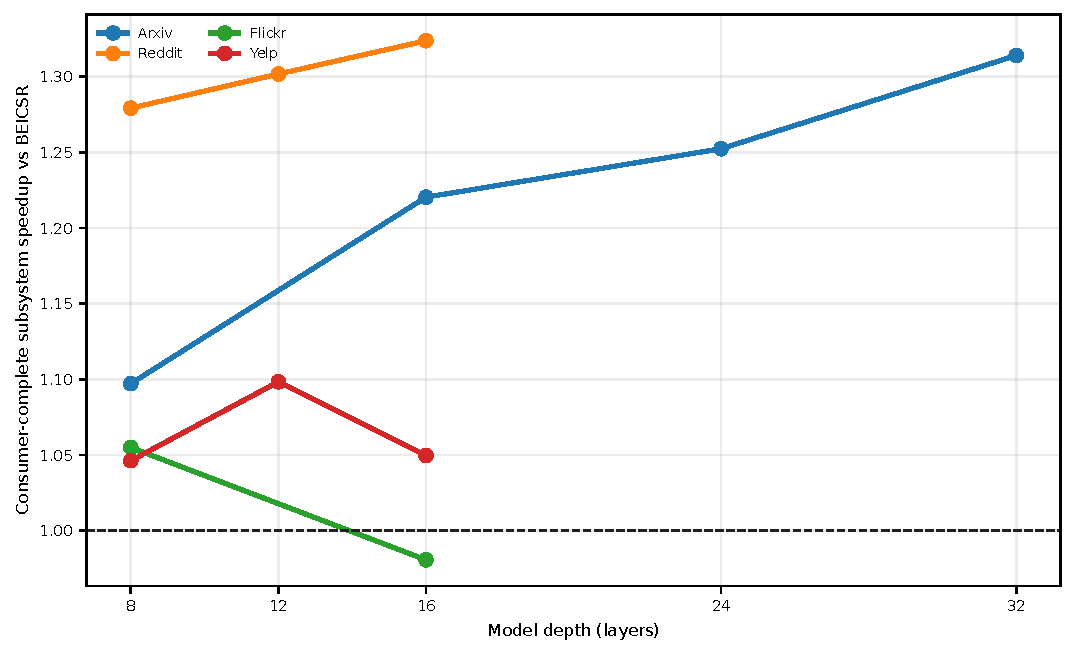
\includegraphics[width=0.78\textwidth]{figures/fig_depth_scaling_consumer_complete.pdf}
\caption{Depthwise consumer-complete sensitivity. Every point is an independently trained model; the D12+ extensions charge producer and consumer anchor recovery and pass exact recurrence checks. Arxiv D24/D32 are borderline-quality diagnostics, Yelp D16 is invalid, and Flickr D16 is a valid negative control; these points do not enter primary aggregates.}
\label{fig:depth-scaling}
\end{figure*}

Figure~\ref{fig:depth-scaling} connects the layerwise persistence in Supplementary Fig.~S1 to subsystem behavior: valid Reddit improves monotonically from 1.279$\times$ at D8 to 1.324$\times$ at D16, while Arxiv exceeds 1.2$\times$ at D16. Flickr's 0.981$\times$ D16 result bounds the claim---depth helps only when positional persistence coincides with exposed memory traffic.

\subsection{Exactness and numerical quality}
Every evaluated stream reconstructs the original support bit-for-bit, so \sys{} adds no numerical error. The paired quality difference comes only from the FP8/FP16 arithmetic shared with the baseline. Across compatible primary checkpoints, FP8/FP16 minus FP32 accuracy ranges from $-0.053$ to $+0.031$ percentage points. Supplementary Table~S6 reports every compatible primary pair; Supplementary Sec.~IX reports the deeper and negative-control configurations.

\subsection{RTL and physical implementation}
\begin{figure*}[t]
  \centering
  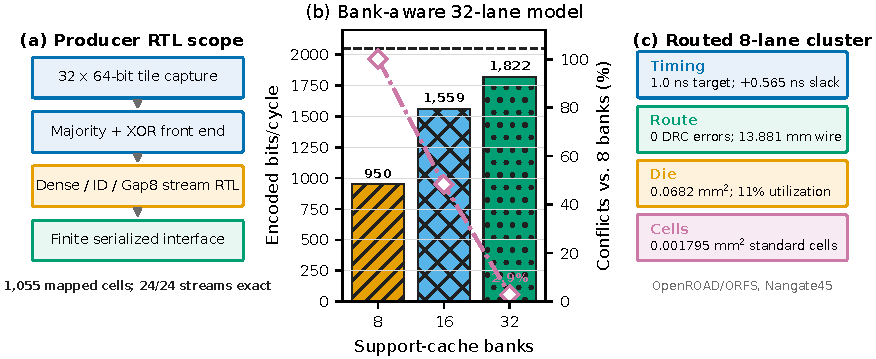
\includegraphics[width=\textwidth]{figures/fig7_implementation_validation.pdf}
  \caption{Implementation evidence. (a) The mapped tile front end performs majority construction and XOR-event discovery; a separate finite stream RTL packs Dense/ID/Gap8 records, while the serialized ready/valid interface matches 24 reference streams. (b) Increasing support-cache banks raises modeled 32-lane throughput from 950 to 1,822 encoded bits/cycle. (c) An integrated eight-lane decoder/support-cache top routes cleanly in Nangate45.}
  \label{fig:implementation}
\end{figure*}

The selector boundary maps to 810 Yosys cells, and the bounded tile front end maps to 1,055 cells. That front end captures a 32-row by 64-feature tile, accumulates the majority mask, discovers XOR events, and exposes a finite ready/valid interface. A separate 2,048-bit stream RTL constructs Dense, fixed-ID, and Gap8 payloads with descriptor offsets; the serialized ready/valid interface reproduces 24 reference streams under randomized stalls. On the consumer side, 32 banks sustain 1,822.4 encoded bits/cycle and reduce conflicts by 97.1\% relative to eight banks. The integrated eight-lane top routes at a 1.0-ns target with +0.565-ns slack, zero detailed-route DRC errors, 13.881~mm of wire, a 0.0682~mm$^2$ die, and 0.001795~mm$^2$ of standard cells. The 16-KiB CACTI support SRAM occupies 0.0549~mm$^2$ with 0.374-ns access and 0.00891~nJ/read.

\subsection{External memory replay}
\label{sec:memoryvalidation}
The internal completion model uses one shared eight-channel resource, but abstracts bank state and row scheduling. Ramulator2 therefore supplies an independent absolute check with HBM2, cache-line interleaving, RoBaRaCoCh mapping, FR-FCFS scheduling, open rows, refresh, and finite read/write queues. The timing scale is calibrated on one complete request stream and evaluated on an independent held-out stream. The model predicts 4,064,919 cycles, while Ramulator2 reports 4,083,428 cycles, an absolute error of 0.453\%. Both streams contain producer reads, consumer-anchor reads, and writebacks, directly testing the shared-memory concurrency abstraction.

DRAMsim3 independently accepts and drains representative real and adversarial streams under a second address mapping. DRAMsim3 confirms complete request service under its independent address mapping. Supplementary Table~S5 reports the held-out comparison, request counts, and the seven SCALE-Sim shapes used by the execution model.

\FloatBarrier
\section{Related Work}

\textbf{Deep residual GNNs and accelerator dataflows.}
Residual and initial-residual formulations such as DeepGCNs and GCNII make substantially deeper GNNs trainable~\cite{li2019deepgcns,chen2020gcnii}. Most GNN accelerators instead target topology irregularity, aggregation--combination imbalance, or dataflow. HyGCN separates sparse aggregation from dense combination~\cite{yan2020hygcn}; GCNAX searches loop order, tiling, and fusion~\cite{li2021gcnax}; ReGNN eliminates redundant message-passing work~\cite{chen2022regnn}; GROW specializes sparse--dense multiplication~\cite{hwang2023grow}; and BeaconGNN reorders storage-side streams~\cite{wang2024beacon}. These mechanisms determine when and where features move, but they do not define a differential representation for positionally aligned supports from successive residual blocks. \sys{} is complementary: it changes the support stream presented to the host dataflow rather than the graph traversal or dense-compute schedule.

\textbf{Sparse and compressed GNN activations.}
SGCN is the closest accelerator precedent. It observes high post-ReLU sparsity in deep residual GCNs, introduces \beicsr{} to encode each feature stream in place, and adds a sparse aggregation path that consumes the compressed representation~\cite{yoo2023sgcn}. \sys{} retains that execution contract and uses an optimized \beicsr{} implementation as its direct baseline, but adds a second redundancy axis: correspondence of support positions across adjacent layers. GNN training systems pursue a different objective. EXACT quantizes activations saved for backpropagation to reduce memory, accepting an accuracy and runtime trade-off, while CompressGNN applies hierarchical compression to reduce training redundancy~\cite{liu2022exact,chen2025compressgnn}. Those methods compress activation state retained for optimization; \sys{} losslessly encodes only the Boolean inference support, leaves packed nonzero values unchanged, and reconstructs the support before irregular aggregation.

\textbf{Activation compression in DNN accelerators.}
SCNN maintains sparse weights and ReLU activations in compressed form, while cDMA compresses sparse activations offloaded during DNN training~\cite{parashar2017scnn,rhu2018cdma}. CompAct uses schedule-aware run-length coding, including sparse and lossy variants, for on-chip CNN activation buffers~\cite{zhang2019compact}. Lossless codecs such as EBPC and Lane Compression exploit bit-plane correlation or small value deltas within one tensor~\cite{cavigelli2019ebpc,ko2021lane}. Transform-based schemes such as JPEG-ACT and the accelerator of Shao et al. compress a feature map transferred between layers, but use lossy spatial transforms and quantization rather than differential coding between two layer outputs~\cite{evans2020jpegact,shao2022interlayer}. Thus, ``interlayer feature-map compression'' in that literature identifies where the compressed tensor sits in the network dataflow; it does not by itself exploit persistence across layer-indexed supports. \sys{} instead operates on aligned Boolean supports and preserves bit-exact inference semantics.

\textbf{Differential and temporal representations.}
Base/delta and XOR constructions are established memory-compression primitives. BDI represents nearby words relative to a base, whereas bit-plane codecs encode local deltas before packing~\cite{pekhimenko2012bdi,cavigelli2019ebpc}. Dynamic-GNN accelerators also exploit change, but along the graph-snapshot axis: Cambricon-DG removes redundant work between evolving graph states~\cite{yue2025cambricondg}. \sys{} applies differential coding along the layer axis of one static-graph inference. Its novelty is not XOR itself, but the causal anchor--target protocol, independently decodable anchor selection, complete-record fallback, fixed-partition non-expansion bound, and explicit producer/consumer anchor lifecycle required to expose reconstructed supports to sparse aggregation.

\section{Conclusion}
\sys{} exploits measured inter-layer support persistence with a causal anchor--delta representation, exact reconstruction, a Hamming-optimal spatial prototype, and complete-record fallback. Across every compatible eight-layer checkpoint, it reduces serialized support writes by 37.1\% and complete physical traffic by 7.9\%. A common finite-queue schedule with explicit producer and consumer anchor recovery, one shared eight-channel read/write memory resource, and SCALE-Sim combination service reaches 1.083$\times$ trace-weighted and 1.076$\times$ dataset-balanced geometric-mean modeled aggregation--combination-subsystem speedup, with a maximum of 1.279$\times$. A held-out Ramulator2 replay validates absolute memory completion within 0.45\%. Producer stream equivalence, bank-aware reconstruction, and a routed eight-lane cluster establish a concrete implementation path. These results show that inter-layer support persistence is a measurable architectural property whose benefit survives causal online encoding, anchor recovery, physical-transfer accounting, shared memory contention, and dense-combination timing.

\balance
\bibliographystyle{IEEEtranS}
\bibliography{refs}

\clearpage
\section*{Appendix: AI Use}
OpenAI ChatGPT (GPT-5.6 Thinking) was used in the following parts of the work. For the Abstract, Introduction, Related Work, and Conclusion, it assisted with organization, sentence-level rewriting, and consistency editing. For the Representation, Analysis, Microarchitecture, and Evaluation sections, it assisted with exposition, notation checks, and integration of author-supplied result tables; the authors independently verified every equation, proof statement, configuration, and numerical claim. It assisted with Python plotting code for Figs.~1--8 and the supplementary figures; the authors checked every plotted point against the packaged source CSV and regenerated the figures locally. It assisted with review-response organization, experiment specifications, and debugging suggestions for evaluation scripts; all experiments were run by the authors, and the authors inspected the source code, tests, logs, and manifests before retaining results. No citation or measurement was accepted without author verification against the supplied source material.

\end{document}
